\setRL
\clearpage
\def \MemDiscr {\Mempath /MembraneDiscrete}

\section{
چکیده
}
در این بخش به روش گسسته سازی انرژی‌های مساحت، حجم، خمش، و الاستیک بر روی شبکه‌های مثلث می‌پردازیم. پس از تعریف گسسته سازی هر انرژی بر مش مثلثی، برای پوسته‌هایی که هم انرژی خمش هم انرژی الاستیک دارند شکل تعادلی مش  و نقطه‌ی بخرانی تغییر شکل بر حسب عدد بی بعد فاپل فون کارمان توضیح داده شده‌است. در آخر نیز روش مثلث بندی دینامیک توضیح داده شده. 



\section{
مقدمه
}
در روش شبیه‌سازی توزیع دینامیک مساحت
\LTRfootnote{Dynamic Area Redistribution}
اندازه و شکل قسمت‌های مِش به طور پیوسته در حال تغییر است. در این مدل تنش بُرشی هزینه‌ی انرژی نداشته و چگالی دولایه‌ی لیپیدی غشا در سراسر مش ثابت فرض شده. در این رساله از شبکه‌ی مثلثی برای پیاده سازی 
Dynamic Area Redistribution (DAR)
استفاده شده‌است. جهت شبیه‌سازی موفق غشا لازم است انرژی مساحت، حجم، و انحنا به درستی در همه نقاط محاسبه شود. صحت معادلات گسسته بر شبکه‌های منظم و تصادفی در مطالعات گذشتگان اثبات شده است (بخش 
\ref{sec:simRevMesh}
). در درجه‌ی اول صحت این معادلات بر شبکه‌های درهم نیز باید اثبات شود. سپس با استفاده از این شبکه‌ها می‌توان رفتار غشا را مطالعه کرد. ابتدا افت و خیز سطح غشای شبیه‌ سازی شده با این روش مطالعه، سپس شکل غشا برای مقادیر مختلف حجم کاهیده بررسی شد. در نهایت در جهت ارائه‌ی کاربرد این مدل، نحوه‌ی تولید گلبول قرمز نمایش داده شده‌است.


\section{
شبکه‌های مثلثی
}

محاسبه‌ی انرژی از طریق مطالعه‌ی افت و خیز سطح روش مناسبی برای بررسی اشکال شبه کُروی است اما برای بررسی عمومی اشکال غیر کروی مشخصات آن باید مستقیم اندازه‌گیری شود. مدل‌های پیوسته‌ی غشا را می‌توان بر روی شبکه‌های مثلثی تعریف کرد. با توزیع یکنواخت نقاط بر روی یک سطح و اتصال هر نقطه  به همسایه‌هایش می‌توان شبکه‌ی مثلثی ساخت. در صورتی که نقاط تنها به همسایه‌های نزدیکشان متصل شوند شبکه‌ی مثلثی تشکیل خواهد شد که هیچ مثلثی در آن با مثلث دیگری همپوشانی ندارد و سطح با مثلث کاملا کاشی می‌شود. شبکه‌های مثلث خواص بسیار جذابی دارند. در شبکه‌‌ی مثلثی تخت با توزیع نقاط یکنواخت، هر نقطه دقیقا ۶ همسایه دارد و آن را با مفهومی به نام درجه‌ی نقطه\LTRfootnote{vertex degree}
بیان کرده و تعداد نقاط با درجه‌ی 
$n$
را با 
$\vartheta_n$
نمایش می‌دهیم. در مورد سطوح با هندسه‌ی بسته یا سطوح با انحنای زیاد تعداد درجات دیگر ثابت نخواهد بود. اویلر نشان داد که اختلاف تعداد  نقاط با درجات ۵ و ۷ برای سطح با هندسه‌ی بسته تابع جینوس
$\chi$
یا مشخصه‌ی اویلر سطح است
\cite{Nguyen2005PRE},
\begin{equation}
\vartheta_D=\vartheta_5-\vartheta_7=12(1-\chi).
\label{eq:vertexDegreeGenus}
\end{equation}
شبکه‌های مثلثی را می‌توان به ۴ گروه شبکه‌ی منظم\LTRfootnote{ordered},
 تصادفی\LTRfootnote{random},
 منظم دَرهَم\LTRfootnote{fluctuating ordered},
 و تصادفی درهم\LTRfootnote{fluctuating random}
دسته بندی کرد. شبکه‌ی منظم شبکه‌ای است با توزیع یکنواخت نقاط که دارای کمترین تعداد نقاط با درجه‌ی به غیر از ۶ است. برای یک کره، طبق رابطه‌ی 
\ref{eq:vertexDegreeGenus}
شبکه‌ی مثلثی است با ۱۲ نقطه با درجه‌ی ۵
$\vartheta_5=12$
و باقی نقاط با درجه‌ی ۶ 
($\vartheta_7=0$).
 در این صورت محل نقاط با درجه‌ی ۵ در گوشه‌های یک ۲۰ وجهی منتظم\LTRfootnote{Icosahedron}
 مماس به کره خواهد بود.
 
 شبکه‌های تصادفی نیز توزیع کم و بیش یکنواختی از نقاط دارند ولی تعداد نقاط با درجه‌ی ۵، ۶، ۷،  و بیشتر در آن بسیار متغیر است. با افزایش دقت در توزیع نقاط بر روی سطح می‌توان درجه‌ی نقاط تشکیل شده را به ۵، ۶، و ۷ محدود کرد. 
 
شبکه‌های درهم منظم یا تصادفی با تغییر توزیع نقاط در شبکه‌های منظم و تصادفی ساخته می‌شوند. توزیع نقاط تحت قیود زیر  پذیرفته می‌شود:

۱) ساختار شبکه‌ی اولیه در فرآیند تغییر مکان نقاط ثابت بماند. به عبارت دیگر توپولوژی شبکه‌ی درهم منظم با توپولوژی شبکه‌ی منظم برابر است.

۲) مثلث‌های جدید حاصل از تغییر توزیع مکان نقاط همچنان سطح را بدون همپوشانی کاشی کند.

%۳) حد کمینه برای اندازه‌ی مثلث‌های تشکیل شده روی سطح قابل تعریف باشد (مثلث با مساحت صفر معنی ندارد).


\section{
تعریف مساحت و حجم
\label{sec:areaVolumeDiscr}
}
\begin{figure}[tbp]
\begin{center}
\includegraphics[width=14cm]{\MemRes/Pics/UnitSphereAreaVolume}
\caption{
مساحت (ستون چپ) و حجم (ستون راست) محاسبه‌ شده برای چهار نوع مش‌های کُروی بر اساس تعداد نقاط روی مش رسم شده‌است. مساحت کل، به دو روش، با جمع مساحت‌های ورنوی (نقاط بنفش) و جمع مساحت‌های بریسنتریک (نقاط خاکستری) محاسبه شده‌است. دقت در اندازه‌گیری مساحت و حجم (نقاط آبی) برای تمام مش‌ها با افزایش تعداد نقاط روی مش، افزایش می‌یابد. تصویر مش نمونه از هر نوع مش استفاده شده در محاسبات کنار هر ردیف رسم شده‌است. به غیر از مش منظم (که تنها یک نمونه از آن برای هر تعداد نقطه وجود دارد) مقادیر محاسبه شده حاصل از میان‌گین گیری بر روی ۵۰ نمونه‌ی مستقل انجام شده‌است.
}
\label{fig:unitsphereAreaVolume}
\end{center}
\end{figure}

جهت بررسی دقت اندازه‌گیری مساحت و حجم برای مش‌های مختلف، مش‌های کروی با تعداد نقاط مختلف انتخاب شد.  مساحت مش‌ها به دو روش محاسبه شد، با جمع  مساحت‌ وُرُنُی رئوس (نقاط بنفش) و جمع مساحت بریسنتریک (نقاط خاکستری). جهت بررسی میزان دقت در اندازه‌گیری،  نتیجه‌ی محاسبات بر مساحت کُره (
$4\pi r_0^2$
)  تقسیم شده‌است. نتایج محاسبات در شکل
\ref{fig:unitsphereAreaVolume}
رسم شده‌است. همانطور که می‌بینید دقت اندازه‌گیری برای تمامی مش‌ها با افزایش تعداد نقاط بهتر می‌شود. لازم به ذکر است  از آنجایی که تمام نقاط مش‌ها روی سطح پوسته‌ی کُروی قرار دارد، یا به عبارت دیگر مش بر داخل یک کره‌ مماس است، مساحت و حجم آن همیشه از کره کمتر خواهد بود.




مشابه به مساحت، حجم نیز برای تمامی مش‌ها با دقت بسیار خوبی قابل اندازه‌گیری‌است. در نتیجه مش‌های درهم برای اندازه‌گیری مساحت و حجم کره مناسب هستند. از آنجایی که غشا‌ها اشکال پیچیده‌تری نسبت به کره دارند، صحت محاسبات برای اشکالی به غیر از کره نیز باید بررسی شود. با اضافه کردن جمله‌ی هارمونیک کروی به مکان شعاعی تمام نقاط مش، می‌توان شکل مش را تغییر داد،
\begin{eqnarray}
r(\theta,\phi)=r_0+r_0|u_{\ell,m}|Y_{\ell,m}(\theta,\phi).
\label{eq:rDeformed}
\end{eqnarray}
با انتخاب
$\ell=2$
و
$m=0$
برای هماهنگ‌ کروی، می‌توان مش‌های دمبلی شکل  تولید کرد. میزان تغییر شکل به شدت مُد
$u_{2,0}$
بستگی دارد. هزینه‌ی انرژی تغییر مساحت یک کره به یک شکل دمبلی طبق معادله‌ی
\ref{eq:AreaGLFluctuationAmplitude}
قابل محاسبه ‌است،
\begin{equation}
E_A=\frac{2}{\pi}|u_{2,0}|^4,
\label{eq:AreaEnergyULM20}
\end{equation}
در معادله‌ی فوق 
$k_A=1[\varepsilon/l^2]$
و
$r_0=1[l]$
فرض شده‌است. نیروی بازگرداننده که با این تغییر شکل مقاومت می‌کند با مشتق گیری از انرژی در فضای مُد قابل محاسبه‌ می‌باشد، 
\begin{equation}
-\frac{\partial E_A}{\partial u_{2,0}}=-\frac{8}{\pi}|u_{2,0}|^3,
\label{eq:AreaForceULM20}
\end{equation}


به همین ترتیب با جایگذاری 
$k_V=1[\varepsilon/l^3]$
در معادله‌ی
\ref{eq:VolumeGLFluctuationAmplitude}
می‌توان انرژی تغییر حجم مش زمانی که از  شکل کره به شکل دمبلی تغییر می‌کند را بر حسب شدت مُد محاسبه کرد،
\begin{equation}
E_V= \frac{3}{8\pi}|u_{2,0}|^4.
\label{eq:VolumeEnergyULM20}
\end{equation}

با مشتق ‌گیری نسبت به شدت مُد، مقدار نیرویی که با تغییر شکل مش مقاومت می‌کند را می‌توان بر حسب شدت مد محاسبه کرد،
\begin{equation}
-\frac{\partial E_V}{\partial u_{2,0}}= -\frac{3}{2\pi}|u_{2,0}|^3,
\label{eq:VolumeForceULM20}
\end{equation}

\begin{figure}[tbp]
\begin{center}
\includegraphics[width=14cm]{\MemRes/Pics/UnitSphereDeformation_mesh_10_Areavolume}
\caption{
انرژی مساحت (ستون 
$(a)$
) و حجم (ستون 
$(b)$
) محاسبه‌ شده حاصل از تغییر شکل مش کروی با اضافه شدن مد
$Y_{2,0}(\theta,\phi)$
با شدت‌های مختلف برای چهار نوع مش رسم شده‌است. انرژی مساحت برای دو روش محاسبه‌ی مساحت کل، جمع مساحت‌های ورنوی (نقاط بنفش) و جمع مساحت‌های بریسنتریک (نقاط خاکستری)، و انرژی حجم (نقاط آبی) با جمع روی حجم هرم‌ها محاسبه شده‌است. خطوط مشکی برای ستون‌های 
$(a)$
و
$(b)$
به ترتیب از رسم معادلات
\ref{eq:AreaEnergyULM20}
و
\ref{eq:VolumeEnergyULM20}
حاصل شده‌است. نیروی بازگرداننده برای تغییر مساحت و حجم در ستون‌های 
$(c)$
و
$(d)$
رسم شده.  پیش‌بینی‌ مرتبه‌ی دوم نیروی بازگرداننده برای تغییر مساحت وحجم با توجه به معادلات
\ref{eq:AreaForceULM20}
و
\ref{eq:VolumeForceULM20}
با خط مشکی رسم شده است. شدت مد 
$u_{2,0}=0$
مربوط به شکل کاملا کروی (عکس سمت چپ) و شدت مد 
$u_{2,0}=1$
مربوط به شکل دمبلی (عکس سمت راست) است. یک نمونه از هر مش برای حالت کروی و دمبلی در ردیف مربوته رسم شده‌است. به غیر از مش منظم (که تنها یک نمونه از آن برای هر تعداد نقطه وجود دارد) مقادیر محاسبه شده حاصل از میان‌گین گیری بر روی ۵۰ نمونه‌ی مستقل انجام شده‌است.
}
\label{fig:unitsphereAreaVolumeULM20}
\end{center}
\end{figure}


در شکل
\ref{fig:unitsphereAreaVolumeULM20}
نتیجه‌ی محاسبات عددی در کنار پیش‌بینی نظری برای انرژی و نیروی حاصل از تغییر شکل رسم شده است. شدت مد
$u_{2,0}=0$
مربوط به مش کاملا کروی است (عکس‌های سمت چپ) و شدت مد 
$u_{2,0}=1$
مربوط به مش‌های دمبلی شکل است (عکس‌های سمت راست). هر ردیف محاسبات را برای یک نوع مش نشان می‌دهد که با  عکسی از آن مش مشخص شده‌است. به ترتیب در ستون‌های 
$(a)$
،
$(b)$
،
$(c)$
، و
$(d)$
تغییر انرژی مساحت، انرژی حجم، نیروی مساحت، و نیروی حجم به صورت نقاط بنفش (ورنوی) و خاکستری (بریسنتریک) برای مساحت و نقاط آبی برای حجم به همراه پیش‌بینی استخراج شده از محاسبات افت و خیز (خط مشکی) رسم شده‌است. 

داده‌های شکل 
\ref{fig:unitsphereAreaVolumeULM20}
نشان می‌دهد که رفتار انرژی و نیرو برای تغییر شکل‌های کوچک با پیش‌بینی مستخرج از محاسبات افت و خیز همخوانی دارد. از آنجایی که محاسبات افت و خیز برای شدت مد‌های کوچک و تا مرتبه‌ی دوم در 
$u_{\ell,m}$
درنظر گرفته شده‌است برای شدت‌ مد‌های بزرگ فاقد اعتبار است. ولی رفتار کلی محاسبات عددی و معادلات
\ref{eq:AreaEnergyULM20}
،
\ref{eq:VolumeEnergyULM20}
،
\ref{eq:AreaForceULM20}
، و
\ref{eq:VolumeForceULM20}
برای شد‌ت مد 
$|u_{\ell,m}|>0.5$
نیز همخوانی دارد. می‌توان نتیجه گرفت که محاسبات لازم برای اندازگیری مساحت و حجم غشا برای شکل‌های کروی و همچنین شکل‌های غیر کروی حاوی انحنای زین اسبی بر روی مش‌های معمولی  و  درهم به خوبی قابل پیاده‌سازی است.













\section{\label{sec:curvatureDiscDef}
تعریف انرژی انحنا
}
\setRL
%\pagenumbering{arabic} 



\subsection{
انرژی خمش بر حسب زاویه‌ی دوسطحی
}
 شبکه‌ی ۲ بعدی مثلثی تحتی را فرض کنید که طول تمام اضلاع آن 
 
 است. در صورتی که صفحه خم شود می‌توان انرژی خم شدن آن را بر حسب بردار عمود بر هر مثلث تعریف کرد،
\begin{equation}
E_b^{discrete}=\frac{1}{2}\epsilon_b\sum_{\langle\alpha,\beta\rangle}|n_\alpha-n_\beta|^2=\epsilon_b\sum_{\langle\alpha,\beta\rangle}\left(1-n_\alpha\cdot n_\beta\right)
\label{eq:bending}
\end{equation}
در اینجا جمع روی تمام جفت‌های 
$n_\alpha$
و 
$n_\beta$ 
است که همسایه‌ی یکدیگر هستند. برای بدست‌ آوردن حد پیوسته‌ فرض می‌کنیم که سطح غشا با پارامتر 
$x(\sigma_i)$
نگاشت شده و محورهای مختصات به صورت 
$e_i=\partial_ix$
تعریف شده که در نتیجه منجر به تعریف متریک و ساختار بنیادی دوم
\LTRfootnote{second fundamental form}
 به ترتیب به صورت 
$g_{ij}=e_i\cdot e_j$
و
$\Omega_{ij}=e_i\cdot\partial_jn$
تعریف می‌شود 
\cite{DubrovinModernGeometry}
. در حد پیوسته اختلاف برداری 
$n_\alpha-n_\beta$
را به صورت گرادیان میدان برداری نوشته می‌شود
\begin{equation}
E_b=\frac{1}{2}\epsilon_b\int dSg^{ij}\partial_in\cdot\partial_jn
%\label{eq:bending}
\end{equation}
با جایگذاری 
$\partial_in\Omega_i^ke_k$
می‌توانیم انرژی خمش را بر حسب 
$\Omega_{ij}$
تعریف کنیم
\begin{equation}
E_b=\frac{1}{2}\epsilon_b\int dSg^{ij}g^{kl}\Omega_{ik}\Omega_{jl}
%\label{eq:bending}
\end{equation}
با استفاده از دو رابطه‌ی 
\begin{equation}
\begin{aligned}
&\epsilon^{il}\epsilon_{jk}=\delta_j^i\delta_k^l-\delta_k^i\delta_j^l\\
&g^{ij}g^{kl}=g^{ik}g^{jl}+\epsilon^{il}\epsilon_{mn}g^{mj}g^{nk}
\end{aligned}
\end{equation}
انتگرالده را به شکل زیر بازنویسی می‌کنیم،
\begin{equation}
\begin{aligned}
g^{ij}g^{kl}\Omega_{ik}\Omega_{jl}&=(g^{ik}\Omega_{ik})^2+\epsilon^{il}\epsilon_{mn}g^{mj}\Omega_{jl}g^{nk}\Omega_{ik}\\
&=(\Omega_i^i)^2+\epsilon^{il}\epsilon_{mn}\Omega_l^m\Omega_i^n=H-2K
\end{aligned}
\end{equation}
که در محاسبات فوق رد
\LTRfootnote{Trace}
 و دترمینان ماتریس فرم بنیادی دوم را با خمش متوسط و خمش گاووسی جایگزاری کردیم،
\begin{equation}
\begin{aligned}
H&=tr\{\Omega_k^i\}\\
K&=\det\{\Omega_k^i\}
\end{aligned}
\end{equation} 
که همان انرژی هلفریش است زمانی که سختی خمش و سختی گوسی قرینه‌ی یکدیگر باشند. اینجا نشان دادیم که با تعریف یک ضریف همبستگی میان مثلث‌های همسایه می‌توانیم رفتار انرژی خمش هلفریش را در سیستم ایجاد کنیم. برای یافتن رابطه‌ی بین ضریب همبستگی مثلث‌های شبکه و سختی خمش هلفریش فرض می‌کنیم استوانه‌ای به طول نامتنهای داریم که انرژی خمش یک نوار از آن به ضخامت
$a$
و شعاع
$R$
به شکل زیر محاسبه می‌شود:
\begin{equation}
\begin{aligned}
E_{continuum}&=\frac{1}{2}\int \kappa H^2dS \\
&=\frac{1}{2}a\kappa\int \frac{1}{R^2}d\ell \\
&=\pi\kappa\frac{a}{R}
\end{aligned}
\label{eq:cylindercontinuum}
\end{equation} 

\begin{figure}[h]
\begin{center}
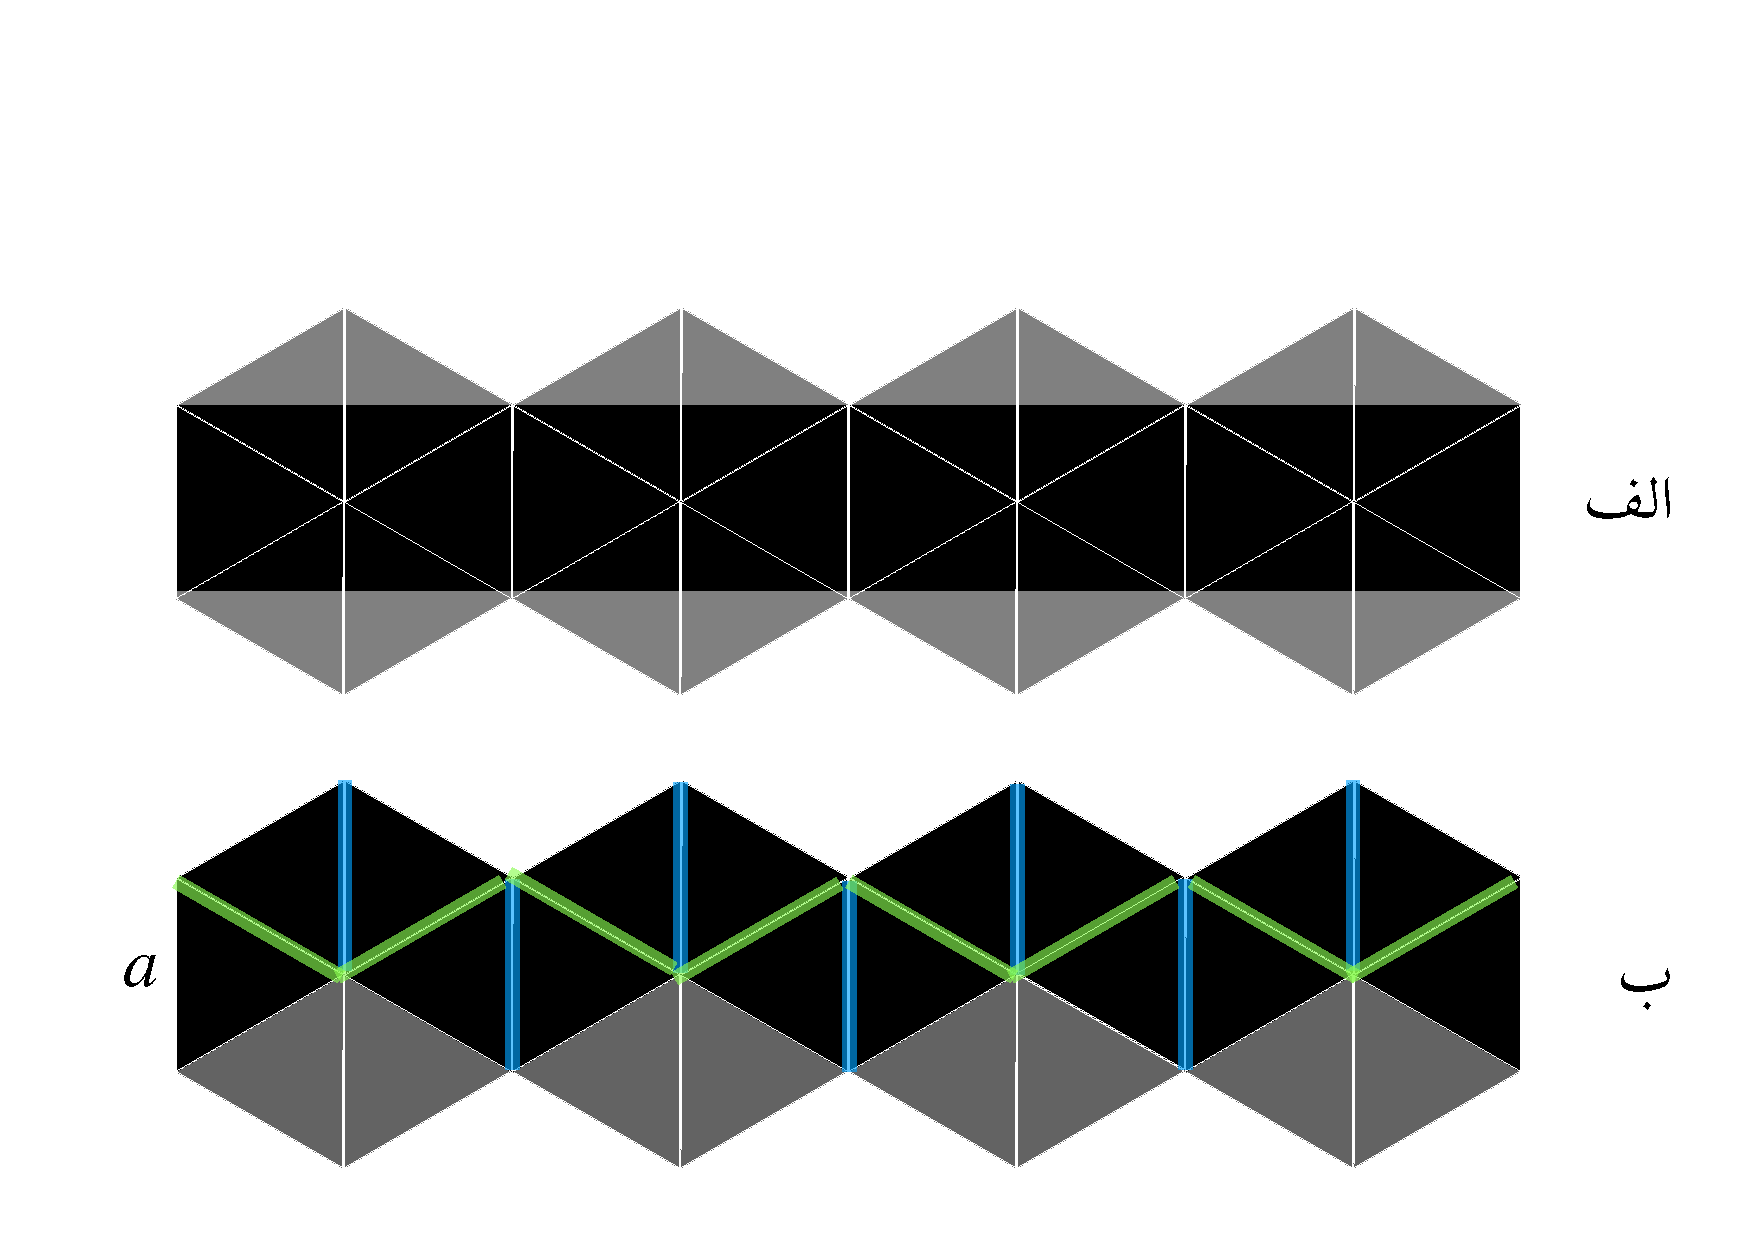
\includegraphics[width=6in]{\MemDiscr/Pics/cylindermesh.pages.pdf}
\caption{
الف، و ب، هر دو نواری از یک شبکه‌ی مثلثی را نشان می‌دهند که هر دو از تعداد یکسان مثلث تشکیل شده‌اند. 
}
\label{fig:cylindermesh}
\end{center}
\end{figure}



ژینوس استوانه برابر ۱ است در نتیجه‌ در محاسبه‌ی انرژي خمش سهمی نخواهد داشت. حال فرض کنید که سطح استوانه را با مثلث (شبکه‌ی نقاط با درجه‌ی ۶) پوشاندیم. شکل
\ref{fig:cylindermesh}
الف، چنین نواری را نشان می‌دهد. اگر فرض کنیم که مثلث‌های نصف شده در بالا و پایین نوار را جابجا کنیم تا مثلث‌های کامل تشکیل شود با شکل
\ref{fig:cylindermesh}
ب، رو برو می‌شویم. اگر این نوار را به دور یک استوانه ببندیم مثلث‌هایی که ضلع مشترک آبی رنگ دارند با یکدیگر زاویه می‌سازند در صورتی که مثلث‌هایی که اضلع مشترک  سبز دارند با یکدیگر زاویه‌ی ۱۸۰ درجه تشکیل می‌دهند. فرض کنیم که طول اضلاع مثلث‌های متساوی الاضلاع 
$a$
 باشد و نوار توسط 
 $N$
 مثلث پوشانده می‌شود. زاویه‌ی میان مثلث‌هایی که ضلع آبی مشترک دارند،
 $\pi\frac{N-2}{N}$
بوده که در نتیجه زاویه‌ی میان بردار‌های عمود به آنها،
 $\pi(1-\frac{N-2}{N})$
خواهد بود. با فرض اینکه تعداد مثلث‌ها به اندازه‌ی کافی بزرگ باشد، انرژی چنین چیدمانی

\begin{equation}
\begin{aligned}
E_{discrete}&=\epsilon_b\sum_{<\alpha,\beta>}\left[1-\cos(\theta_{\alpha,\beta})\right]\\
&=2N\epsilon_b\left[1-\cos\left(\pi(1-\frac{N-2}{N})\right)\right]\\
&=2N\epsilon_b\left[1-\left(1-\frac{1}{2}\left(\pi(\frac{2}{N}\right)^2\right)\right]\\
&=N\epsilon_b\left[\frac{\pi^2}{2}\left(\frac{2}{N}\right)^2\right]\\
&=\frac{4\pi^2}{N}\epsilon_b
\end{aligned}
\label{eq:cylinderdiscrete}
\end{equation} 
در حد 
$N$
های خیلی بزرگ معادله‌ی 
\ref{eq:cylinderdiscrete}
 و 
\ref{eq:cylindercontinuum}
باید پاسخ یکسان داشته باشند. از طرفی محیط سطح مقطع دایره‌ای استوانه با تعداد مثلث‌ها و طول ضلع آن رابطه دارد،
\begin{equation}
\begin{aligned}
2 \pi R &= \frac{N}{2}\frac{\sqrt3}{2}a\\
\frac{a}{R}&=\frac{8}{\sqrt3}\frac{\pi}{N}
\end{aligned}
\label{eq:cylinderdiscretisation}
\end{equation} 
برابر قرار دادن انرژي حد پیوسته و گسسته و جایگاذاری نسبت ضلع مثلث به شعاع استوانه از معادله بالا ما را به رابطه‌ی میان سختی خمش هلفریش و ضریب جفت شدگی مثلث‌ها می‌رساند:
\begin{equation}
\begin{aligned}
\pi\kappa\frac{a}{R}&=4\frac{\pi^2}{N}\epsilon_b\\
\pi\kappa\frac{8}{\sqrt3}\frac{\pi}{N}&=4\frac{\pi^2}{N}\epsilon_b\\
\kappa&=\frac{\sqrt{3}}{2}\epsilon_b
\end{aligned}
\label{eq:epsilonkappa}
\end{equation} 




.
 
 
 
 
 
 
 
 
 
 
 
 
 
 
 
\setRL
%\pagenumbering{arabic} 



\subsection{
انرژي خمش متوسط
}


خمش متوسط یک ناحیه روی مِش 
$H=C_1+C_2$
جمع خمش‌های اصلی در آن نقطه است. در این صورت می‌توان انرژی خمش را با جمع خمش میانگین در هر نقطه تعریف کرد،
\begin{eqnarray}
E_{b}=\frac{1}{2}\kappa\int dA \left[H-C_0\right]^2\equiv\frac{1}{2}\kappa\sum_i a_i \left[H_i-C_0\right]^2,
\label{eq:bendingDiscretisation}
\end{eqnarray}
در اینجا 
$H_i$
، خمش متوسط در هر نقطه،  
$v_i$
است، 
$C_0$
عکس شعاع خمش،  و 
$a_i$
سهم مساحتی است که هر نقطه روی سطح دارد. شعاع خمش متوسط در هر نقطه را می‌توان بر اساس مساحت هر نقطه به شکل 
$H_i=\frac{h_i}{a_i}$
 در نظر گرفت، و معادله‌ی بالا را بازنویسی کرد،
\begin{eqnarray}
\begin{aligned}
E_{b}&=\frac{1}{2}\kappa\sum_i a_i \left[\frac{h_i}{a_i}-C_0\right]^2\\
&=\frac{1}{2}\kappa\sum_i a_i \left[\frac{h_i^2}{a_i^2}-2\frac{h_i}{a_i}C_0+C_0^2\right]\\
&=\frac{1}{2}\kappa\sum_i \left[\frac{h_i^2}{a_i}-2h_iC_0+a_iC_0^2\right]
\end{aligned}
\label{eq:bendingDiscretisationSpontaneous}
\end{eqnarray}
در صورتی که خمش ذاتی برابر صفر باشد، 
\begin{equation}
E_{b}=\frac{1}{2}\kappa\sum_i \frac{h_i^2}{a_i}
\end{equation}


\subsubsection{
روش ایتزیکسون
}
در بخش قبل نحوه‌ی محاسبه‌ی انرژی خمش به روش دو سطحی
\LTRfootnote{dihedral}
معرفی شد. این روش در اصل توسط نلسون و کانتور
\cite{NelsonPRL1987}
معرفی شده بود. گامپر و کرول در سال ۱۹۹۶ به طور مفصل این روش را نقد کرده‌اند
\cite{Gompper1996}
. این روش مشکلات زیادی دارد که در واقع خمش شکل را غلط پیشبینی می‌کند. مشکل اساسی این است که رابطه‌ی 
$\epsilon_b$
و 
$\kappa$
(معادله‌ی  
\ref{eq:HelfrichCurvatureEnergy}
) تابع شکل سطح است.  مثلا برای کره
$\epsilon_b\approx\frac{\sqrt{3}}{2}\kappa$
و برای استوانه
$\epsilon_b\approx\sqrt{3}\kappa$
است. پس نمی‌توان از این رابطه برای محاسبه‌ی سطحی که در حال تغییر شکل است و یا شکل خوش تعریفی ندارد استفاده کرد. 
از طرف دیگر از آنجایی که این انرژی تنها میان یک جفت مثلث تعریف می‌شود و از هندسه‌ی اطرافش بی‌خبر است، نمی‌تواند انرژی نقاط زین اسبی را به درستی محاسبه کند. و در نهایت اندازه‌ی مثلث‌ها در اندازه‌ی خمش نقشی ندارند. این نکته از طرفی مهم است زیرا انرژی خمش مستقل از اندازه‌ی هندسی شکل است ولی در حالتی که مش مثلث‌های با اندازه‌های مختلف داشته باشد، یک جفت مثلث غول‌آسا و یک جفت مثلث ریز به یک می‌زان انرژی خمش خواهند داشت.

\begin{figure}[h]
\begin{center}
\includegraphics[width=4.5in]{\MemDiscr /Pics/tringlePairBoth}
\caption{
سمت چپ زاویه‌های 
$\theta_1^{ij}$
و
$\theta_2^{ij}$
را نشان می‌دهد که زاویه‌هایی است که در شبکه‌ی دوگان به ضلع
$\ell_{ij}$
نسبت داده می‌شود
\cite{Meyer2003}
. سمت راست جفت مثلثی همراه بردار‌های عمود بر سطوح آن،
$n_\alpha$
و
$n_\beta$
و زاویه‌ی دوسطحی میان آن دو
$\phi_{ij}$
نمایش داده شده ‌است.
}
\label{fig:trianglePairAngle}
\end{center}
\end{figure}

ایتزیکسون
\LTRfootnote{Itzykson}
در سال ۱۹۸۶ لاپلاسین میدان اسکالر بر روی یک شبکه‌ی مثلثی تصادفی را ب محاسبه کرد
\cite{Itzykson1986}

از طرفی طبق هندسه‌ی دیفرانسیلی  خمش متوسط در هر نقطه 
$\vec r$
که بردار عمود بر سطح 
$\vec n$
را دارد به شکل 
$H=\vec n\cdot\Delta \vec R$
تعریف می‌شود 
\cite{Gompper1996}
و 
$\Delta$
عملگر لاپلاس بلترامی 
\LTRfootnote{Laplace–Beltrami}
است. 


گامپر و کرول در سالت ۱۹۹۲ از رابطه‌ی ایتزیکسون برای محاسبه‌ی خمش بر روی یک شبکه‌ی مثلثی استفاده کردند،
\begin{eqnarray}
E_{b}^{I}=\frac{1}{2}\kappa\sum_{i}\frac{1}{\sigma_i}\left[\sum_{j(i)}\frac{\tilde\ell_{ji}}{\ell_{ij}}(\vec r_i-\vec r_j)\right]^2.
\label{eq:ItzyksonPotential}
\end{eqnarray}

در اینجا 
$\ell_{ij}$
طول ضلع تعریف شده میان نقاط 
$i$
و
$j$
است، 
$\vec r_i$
و
$\vec r_j$
بردار‌های مکان نمای این دو نقطه‌ است (شکل
\ref{fig:trianglePairAngle}
). 
$\tilde\ell_{ij}$
طول ضلع 
$\ell_{ij}$
در شبکه‌ی دوگانه‌ 
\LTRfootnote{dual lattice}
است و با استفاده از زوایا‌ی روبرو آن به شکل 
\begin{eqnarray}
\tilde\ell_{ij}=\frac{1}{2}\ell_{ij}(\cot\theta_1^{ij}+\cot\theta_2^{ij})
\label{eq:dualLattice}
\end{eqnarray}
تعریف می‌شود.

\begin{figure}[htbp]
\begin{center}
\includegraphics[width=9cm]{\MemDiscr /Pics/Voronoi_Barycentric}

\caption{
سمت چپ مساحت بریسنتریک (مرکز جرمی) و سمت راست مساحت وُرُنُوی برای یک پلاکت را نمایش می‌دهد.
}
\label{fig:voronoiBarycentric}
\end{center}
\end{figure}
مساحت وُرُنُوی
\LTRfootnote{Voronoi}
یک نقطه به اندیس 
$i$
با استفاده از طول اضلاع در شبکه‌ی دوگانی قابل محاسبه است
\begin{eqnarray}
\sigma_i=\frac{1}{4}\sum_{j(i)}\tilde\ell_{ij}\ell_{ij}.
\label{eq:voronoiArea}
\end{eqnarray}
. در معادله‌ی بالا جمع روی تمام اندیس‌های همسایه‌ی نقطه‌ی 
$i$
است. با توجه به این تعاریف در هر نقطه می‌توان خمش را به شکل زیر تعریف کرد،
\begin{eqnarray}
H_i=\vec n\cdot\Delta \vec r\equiv\frac{1}{\sigma_i}\vec n \cdot\left[\frac{\sum_{j(i)}\tilde\ell_{ji}}{\ell_{ij}}(\vec r_i-\vec r_j)\right],
\label{eq:meanCurvatureDiscreteSingleVertex}
\end{eqnarray}
. تعریف بردار عمود در هر نقطه به شکل زیر تعریف می‌شود
\cite{Thurrner1998NormalVec}
\begin{eqnarray}
\vec n_i=\frac{\sum_{tri(i)} \eta_{tri}^i~\vec n_{tri}^i}{|\sum_{tri(i)} \eta_{tri}^i~\vec n_{tri}^i|},
\label{eq:noramlVector}
\end{eqnarray}
که جمع روی تمام مثلث‌های عضو پلاکت
\LTRfootnote{placket}
است (تمام مثلث‌هایی که نقطه‌ی 
$i$
بین آنها مشترک است). 
$\eta_{tri}^i$
و
$\eta_{tri}^i$
به ترتیب زاویه‌ی راس مثلث در نقطه‌ی 
$i$
و بردار عمود بر مثلث است. از آنجایی که در ۳ بُعد بردار عمود بر سطح و لاپلاسین هم‌جهت هستند
\cite{Gompper1996}
معادله‌ی 
\ref{eq:ItzyksonPotential}
تعریف صحیحی از خمش است. تعریف خمش در هر نقطه در صورتی که نیاز به  اضافه کردن خمش ذاتی به معادله خمش باشد، اهمیت دارد. 

معادله‌ی
\ref{eq:ItzyksonPotential}
برای شبکه‌های مثلثی در نظر گرفته شده که مثلثی با زاویه‌ی منفرجه نداشته باشد و همچنین شکل و اندازه تمام مثلث‌ها تقریبا یکسان باشد
\cite{Itzykson1986}
. همانطور که گامپر و کرول هم اشاره کرده‌اند
\cite{Gompper1996}
در این روش داشتن زوایای منفرجه ناپایداری‌های عددی در محاسبات خمش (به خصوص در علامت پارامتر‌های 
$\sigma_i$
یا
$\tilde\ell_{ij}$
) ایجاد خواهد کرد. به این علت مهم، این روش تنها  در مطالعاتی به کار برده می‌شود  که مِش‌های  مثلثی  توزیع یکنواختی از نقاط داشته و توزیع طول اضلاع کنترل شده باشد تا تمام مثلث‌های تشکیل شده اندازه و شکل کم و بیش یکسان داشته باشند.



\subsubsection{
روش یولیشِر
}
۱۰ سال پس از ایتزیکسون، در سال ۱۹۹۶ فرنک یولیشِر 
\cite{Julicher1996}
روش دیگری برای تخمین خمش بر نقاط شبکه‌های مثلثی استفاده کرد. در روش یولیشِر خمش متوسط در هر نقطه با محاسبه‌ی  میانگین تصویر تانسور خمش برای هر دوسطحی (جفت مثلث‌) بر صفحه‌ی مماس بر پلاکت  تخمین زده می‌شود
\cite{Ramakrishnan2011}
مساحت بَرییسنتریک
\LTRfootnote{Barycentric}
(مرکز جرمی) سهم هر نقطه را در خمش تعیین می‌کند،
\begin{eqnarray}
E_{b}^{J}=2\kappa\sum_{i}\frac{1}{a_i}\left[\sum_{j(i)}\frac{1}{4}(\ell_{ij}\phi_{ij})\right]^2.
\label{eq:JulicherPotential}
\end{eqnarray}
در معادله‌ی بالا 
$\ell_{ij}$
و
$\phi_{ij}$
طول ضلع و زاویه‌ی دوسطحی آن (شکل
\ref{fig:trianglePairAngle}
) است. با فرض اینکه توپولوژی سطح تغییر نکند، مشخصه‌ی اویلری سطح ثابت باشد، و سطح خمش ذاتی نداشته باشد، خمش ذاتی میانگین سطح با جمع زیر محاسبه می‌شود، 
\begin{eqnarray}
M=\frac{1}{2}\sum_{<i,j>)}\ell_{ij}\phi_{ij} = \frac{1}{4}\sum_i\sum_{j(i)}\ell_{ij}\phi_{ij}.
\label{eq:JulicherTotalMeanCurvature}
\end{eqnarray}
مساحتی که به هر نقطه نسبت داده می‌شود،
$a_i$
مساحت بریسنتریک (مرکز جرمی) پلاکت است (شکل
\ref{fig:voronoiBarycentric}
) که برابر یک سوم مساحت تمام مثلث‌های پلاکت است، 
\begin{eqnarray}
a_i=\frac{1}{3}\sum_{tri (i)}a_{tri}.
\label{eq:BarycentricArea}
\end{eqnarray}
در این مدل، در صورتی که خمش ذاتی در سطح وجود داشته باشد، خمش در هر نقطه به شکل،
\begin{eqnarray}
H_i^J=\vec n\cdot\frac{1}{4}\frac{1}{a_i}\sum_{j(i)}\ell_{ij}\phi_{ij},
\label{eq:meanCurvatureDiscreteSingleVertexJulicher}
\end{eqnarray}
تعریف می‌شود. در اینجا تعریف بردار عمود بر سطح مطابق معادله‌ی
\ref{eq:noramlVector}
است. رابطه‌ی یولیشر را با یک فاکتورگیری ساده می‌توان مشابه با رابطه‌ی ایتزیکسون بازنویسی کرد،
\begin{eqnarray}
E_{b}^{J}=\frac{1}{2}\kappa\sum_{i}\frac{1}{a_i}\left[\sum_{j(i)}\frac{1}{2}(\ell_{ij}\phi_{ij})\right]^2.
\label{eq:JulicherPotentialHalf}
\end{eqnarray}
در قسمت نتایج نشان خواهیم داد که اختلاف خمش میانگین محاسبه شده توسط ایتزیکسون و یولیشر در وزنی‌است که به هر پلاکت نسبت می‌دهند و برای عموم چیدمان‌ پلاکت‌ها و خمش سطح کوچک،
\begin{eqnarray}
\left[\sum_{j(i)}\frac{1}{2}(\ell_{ij}\phi_{ij})\right]^2\approx\left[\sum_{j(i)}\frac{\sigma_{ij}}{\ell_{ij}}(\vec r_i-\vec r_j)\right]^2.
\label{eq:JulicherItzyksonNumerator}
\end{eqnarray}


\subsubsection{
روش‌های ایتزیکسون-بریسنتریک و یولیشر-ورنوی
}
با توجه به رابطه‌ی 
\ref{eq:JulicherItzyksonNumerator}
با جابجایی وزن نسبت داده شده به هر پلاکت می‌توان دو نوع روش جدید برای محاسبه‌ی خمش در شبکه‌های مثلثی طراحی کرد. یکی محاسبه‌ی خمش به روش ایتزیکسون ولی با وزن بریسنتریک،
\begin{eqnarray}
E_{b}^{IB}=\frac{1}{2}\kappa\sum_{i}\frac{1}{a_i}\left[\sum_{j(i)}\frac{\sigma_{ij}}{\ell_{ij}}(\vec r_i-\vec r_j)\right]^2,
\label{eq:ItzyksonBarycentricPotential}
\end{eqnarray}
و دیگری محاسبه‌ی خمش با روش یولیشر ولی با وزن ورنوی است،
\begin{eqnarray}
E_{b}^{JV}=\frac{1}{2}\kappa\sum_{i}\frac{1}{\sigma_i}\left[\sum_{j(i)}\frac{1}{2}(\ell_{ij}\phi_{ij})\right]^2.
\label{eq:JulicherVoronoiPotential}
\end{eqnarray}
انگیزه‌ی اصلی برای پیشنهاد این دو روش جدید بررسی پایداری عددی روش‌های مختلف محاسبه‌ی خمش برای محاسبات دینامیک ملکولی است.  در بخش نتایج مفصل راجع به پایداری عددی این روش‌ها صحبت خواهد شد.








 

\section{
تعریف انرژی کششی
\label{sec:youngMesh}
}
\setRL
%\pagenumbering{arabic} 

\subsection{
انرژي آزاد کشش
}

در نظریه‌ی الاستیک سطح هر تغییر شکل با یک میدان بردار جابجایی 
$u(r)=(u_1,u_2)$
نشان داده می‌شود نقطه‌ی 
$r(x,y)$
را به نقطه‌ی 
$r+u$
نگاشت می‌کند. اگر در شبکه نقص وجود نداشته باشد این نگاشت یک به یک خواهد بود. در صورتی که فرض کنیم که ماده مورد مطالعه یکنواخت و همسانگرد است، برای جابجایی‌های کوچک (رژیم خطی) قانون هوک را به شکل توان دوم تانسور کرنش نوشت
\LTRfootnote{Cauchy, 1822; Lam ́e, 1852}
،
\begin{equation}
E_s=\frac{1}{2}\int d^2r(2\mu u_{ij}^2+\lambda u_{kk}^2)
\label{eq:energylame}
\end{equation}
که در اینجا $\lambda$
و $\mu$
ثابت‌های لم
\LTRfootnote{Lamé Coefficients}
است. ما می‌دانیم که تانسور کرنش به شکل زیر تعریف می‌شود،
\begin{equation}
u_{ij}=\frac{1}{2}(\partial_i u_j+\partial_j u_i+\partial_i u_k\partial_j u_k)
\end{equation}
اما برای جابجایی کوچک از جمله‌ی غیر خطی صرف نظر می‌کنیم و تانسور کرنش را به این شکل تعریف می‌کنیم.
\begin{equation}
u_{ij}=\frac{1}{2}(\partial_i u_j+\partial_j u_i)
\label{eq:simplestrain}
\end{equation}
می‌توانیم  از انرژی کششی گرادیان بگیریم و مقدار کمینه‌ی آن را بررسی کنیم، در نتیجه
\begin{equation}
\begin{aligned}
&\partial_i\sigma_{ij}=0\\
&\sigma_{ij}=2\mu u_{ij}+\lambda u_{kk}\delta_{ij}
\label{eq:stress}
\end{aligned}
\end{equation}
که در این معادله 
$\sigma_{ij}$
تانسور تنش است. معادله‌ی 
\ref{eq:stress}
را به تنهایی می‌توان حل کرد ولی از آنجایی که دیورژانس تنش صفر است معمول است که این معادله را به شکل یک پتانسیل اسکالر بنویسیم،
\begin{equation}
\sigma_{xx}=\frac{\partial^2\chi}{\partial y^2},\quad\sigma_{yy}=\frac{\partial^2\chi}{\partial x^2},\quad\sigma_{xy}=\frac{\partial^2\chi}{\partial_x\partial_y} 
\end{equation}
انتخاب‌های خیلی زیادی می‌توانند معادله‌ی بالا را ارضاء خواهد کرد، ولی جواب‌هایی که به لحاظ فیزیک قابل قبول هستند باید بتوانند رابطه‌ی بین میدان جابجایی و 
$\chi$
را رعایت کنند،
\begin{equation}
\begin{aligned}
\frac{1}{2}(\partial_iu_j+\partial_ju_i)&=u_{ij}\\
&=\frac{1+\nu}{Y}\sigma_{ij}-\frac{\nu}{Y}\sigma_{ll}\sigma_{ij}\\
&=\frac{1+\nu}{Y}\epsilon_{im}\epsilon_{jn}\partial_{m}\partial_{n}\chi-\frac{\nu}{Y}\nabla^2\chi\delta_{ij}
\label{eq:constraint}
\end{aligned}
\end{equation}
در اینجا $Y$
و $\nu$
به ترتیب مدول ۲ بعدی یانگ
\LTRfootnote{2D Young Modulus}
 و نسبت پواسون
\LTRfootnote{Poisson ratio}
است که بر حسب ضرایب لم به شکل زیر بیان می‌شوند،
\begin{equation}
\begin{aligned}
Y&=\frac{4\mu(\mu+\lambda)}{2\mu+\lambda}\\
\nu&=\frac{\lambda}{2\mu+\lambda}
\label{eq:younglame}
\end{aligned}
\end{equation}
فرض می‌کنیم که شبکه‌ای را بررسی می‌کنیم که فاصله‌ی متوسط بین تمام نقاط به اندازه‌ی $a$ باشد. هر گونه تغییر شکل در شبکه یک نقطه از شبکه را از $r_a$ به $r_a'$ جابجا خواهد کرد. در نتیجه می‌توان انرژی کشش را به شکل زیر تعریف کرد (شکل
\ref{fig:mesh_def}
).
\begin{figure}[h]
\begin{center}
\includegraphics[width=6in]{\MemModel/Pics/mesh_def.pages.pdf}
\caption{
تغییر شکل مش
}
\label{fig:mesh_def}
\end{center}
\end{figure}

\begin{equation}
E_s^{discrete}=\frac{1}{2}\epsilon_s\sum_{\langle a,b\rangle}\left(|r_a'-r_b'|-a\right)^2
\label{eq:stretchdiscrete}
\end{equation}
که جمع روی تمام جفت‌های $a$ و $b$ است که شامل تغییر شکل شده‌اند.  همچنین می‌توان جمع بالا را به شکل چگالی موضعی انرژی حول نقاط شبکه و جمع روی همسایگی‌ آن نقاط تعریف کرد،

\begin{equation}
\begin{aligned}
&E_s^{discrete}=\frac{1}{2}\epsilon_s\sum_aU_a\\
&U_a=\frac{1}{2}\sum_b\left(|r_a'-r_b'|-a\right)^2
\end{aligned}
\end{equation}
برای محاسبه‌ی حد پیوستگی فرض می‌کنیم که نقشه‌‌ی تغییر شکل پیوسته‌ای وجود دارد که نقاط 
$r\rightarrow r'$
که معادل نقشه‌ی گسسته‌ی شبکه‌ی ماست
$r_a\rightarrow r_a'=r_a+u_a(r_a)$
. اگر تانسور متریک این تغییر شکل به شکل زیر تعریف شده باشد،
\begin{equation}
g_{ij}=\partial_i r'\cdot\partial_jr'
\end{equation}
در نتیجه می‌توانیم تغییر شکل گسسته را به شکل زیر تخمین بزنیم،

\begin{equation}
\begin{aligned}
|r_a'-r_b'|&\approx \left[g_{ij}(r_a)r_{ab}^ir_{ab}^j\right]^{1/2}\\
&= \left[g_{ij}(r_a)r_{ab}^ir_{ab}^j\right]^{1/2}\\
&= \left\{\left[\delta_{ij}+2u_{ij}(r_a)\right]r_{ab}^ir_{ab}^j\right\}^{1/2}\\
&= a\left[1+2u_{ij}(r_a)\frac{r_{ab}^ir_{ab}^j}{a^2}\right]^\frac{1}{2}\\
&\approx a\left[1+u_{ij}(r_a)\frac{r_{ab}^ir_{ab}^j}{a^2}\right]
\label{eq:gstrain1}
\end{aligned}
\end{equation}
که در رابطه‌ی بالا تانسور متریک را با تانسور تنش جاگذاری کردیم،
$g_{ij}=\delta_{ij}+2u_{ij}$
از آنجایی که اندیس $b$ بین تمامی همسایه‌ی $a$ تعریف می‌شود و همچنین بردار فاصله‌
$r_{ab}=r_a-r_b$
روی بردار‌های
$d_\beta$
 شبکه‌ی شش ضلعی تعریف می‌شود می‌توانیم انرژی موضعی را به این ترتیب محاسبه‌ کنیم،

\begin{equation}
\begin{aligned}
U_a&=\frac{1}{2}\sum_{\beta=1}^6(u_{ij}\frac{d_\beta^id_\beta^j}{a})^2\\
&=\frac{1}{2a^2}\sum_{\beta=1}^6u_{ij}u_{kl}d_\beta^id_\beta^jd_\beta^kd_\beta^l\\
&=\frac{1}{2a^2}a^2u_{ij}u_{kl}(\delta_{ij}\delta_{kl}+\delta_{ik}\delta_{jl}+\delta_{il}\delta_{jk})\cos^2(\pi/3)\\
&=\frac{3}{8}(2u_{ij}^2+u_{kk}^2)
\label{eq:gstrain1}
\end{aligned}
\end{equation}
در نتیجه‌ حد پیوسته انرژی کشسانی را می‌توان به شکل زیر نوشت
\begin{equation}
\begin{aligned}
E_s^{discrete}=\frac{1}{2}\epsilon_s\sum_\alpha U_a&\approx\frac{1}{\sqrt3}\epsilon\int d^2rU(r)\\
&\approx\frac{\sqrt3}{8}\epsilon_s\int d^2r(2u_{ij}^2+u_{kk}^2)
\end{aligned}
\end{equation}
با مقایسه با معادله‌ی 
\ref{eq:energylame}
می‌توانیم ضرایب لم را بخوانیم
\begin{equation}
\lambda=\mu=\frac{\sqrt3}{4}\epsilon_s
\end{equation}
با داشتن ضرایب لم می‌توانیم با توجه به معادله‌ی 
\ref{eq:younglame}
مدول ۲ بعدی یانگ و ضریب پواسون را برای این شبکه محاسبه کنیم،
\begin{equation}
\begin{aligned}
Y&=\frac{4\mu(\mu+\lambda)}{2\mu+\lambda}=\frac{2}{\sqrt3}\epsilon_s\\
\nu&=\frac{\lambda}{2\mu+\lambda}=\frac{1}{3}
\end{aligned}
\end{equation}
همانطور که می‌بینیم برای مش‌های مثلثی ۶ ضلعی، مدول یانگ و نسبت پواسون به اندازه‌ی مش بستگی ندارد. محاسبات عددی
\cite{springnetworkPRE2011}
نیز این نتایج را تایید می‌کنند.




.
 
 
 
 
 
 
 
 
 
 
 
 
 
 
 

\section{
تغییر انرژی آزاد با افزودن نقطەی نقص به شبکه
}
\subsection{
تغییر انرژی کششی
}


در نظریه‌ی الاستیک سطح هر تغییر شکل با یک میدان بردار جابجایی 
$u(r)=(u_1,u_2)$
نشان داده می‌شود نقطه‌ی 
$r(x,y)$
را به نقطه‌ی 
$r+u$
نگاشت می‌کند. اگر در شبکه نقص وجود نداشته باشد این نگاشت یک به یک خواهد بود. در صورتی که در شبکه دررفتگی
\LTRfootnote{dislocation}
یا نقص وجود داشته باشد هر انتگرال بسته پاد ساعتگرد که محل نقص داخل آن قرار گیرد با بردار ثابت برگر
\LTRfootnote{Burger}
برابر خواهد بود.
\cite{mitchell1961}
از آنجایی هم که بردار برگر همیشه با یکی از بردارهای شبکه برابر است، یک به یک نبودن نگاشت در حضور نقص مشکلی در فیزیک مسئله ایجاد نخواهد کرد. این بحث به زبان ریاضی شکل زیر را به خود می‌گیرد،
\begin{equation}
\begin{aligned}
&\oint_Ldu_k=\oint_L\partial_iu_kdx_i=b_k\\
&\epsilon_{li}\partial_l\partial_iu_j=b_j\delta(r-r_0)
\end{aligned}
\end{equation}
که در بالا 
$r_0$
محل نقص، و 
$b$
 بردار برگر است. در رفتگی  بر حسب میدان زاویه‌ی بین پیوندهای شبکه مشخص می‌شود، که جهت گیری در پیرامون هر اتم را مشخص می‌کند. صراحت هر نقص،
 $s$
 حول هر مسیر بسته دور نقص تعریف می‌شود. در شبکه‌ای که تقارن $n$
 تایی داشته باشد، 
 $s$ حتما ضریبی از 
 $2\pi/n$ خواهد بود.
 در این بخش شبکه‌های شش ضلعی با تقارن 
 $n=6$
و لغزش‌های کوچک
$s=\pm2\pi/6$
مورد توجه ماست. به زبان ریاضی می‌توان این جملات را به این شکل نشان داد،

 \begin{equation}
\begin{aligned}
&\oint_Ld\theta=\oint_L\partial_i\theta dx_i=s\\
&\epsilon_{ij}\partial_i\partial_i\theta=s\delta(r-r_0)
\label{eq:thetauij}
\end{aligned}
\end{equation}
با جایگذاری
\begin{equation}
\theta=\frac{1}{2}\epsilon_{ij}\partial_iu_j
\end{equation}
حال می‌خواهیم شرایط معادله‌ی 
\ref{eq:constraint}
را به صورت قید برای $\chi$
تعریف کنیم تا تضمین کند که همیشه می‌توانیم $\chi$
را به صورت جابجایی‌ها بنویسیم. برای اینکار طرفین معادله‌ی 
\ref{eq:constraint}
را در 
$\epsilon_{ik}\epsilon_{jl}\partial_k\partial_l$
ضرب می‌کنیم که نتیجه‌ی آن،
\begin{equation}
\frac{1}{Y}\nabla^4\chi=\epsilon_{ik}\epsilon_{jl}\partial_k\partial_lu_{ij}=\epsilon_{ik}\epsilon_{jl}\partial_k\partial_l\frac{1}{2}(\partial_iu_j+\partial_ju_i)
\label{eq:incompatibility}
\end{equation}
در صورتی که سمت راست معادله‌ی فوق برابر با صفر شود، می‌توان گفت که $u_{ij}$ 
سازگار است و تنها یک جواب برای میدان جابجایی وجود دارد که جواب معادله‌ی 
\ref{eq:constraint}
است. در غیر این صورت معدله‌ی 
\ref{eq:constraint}
بیش از یک جواب دارد. در نتیجه رایج است که به نام سمت راست معادله‌ی
\ref{eq:incompatibility}
را ناسازگاری
\LTRfootnote{incompatibility}
و $\epsilon_{ik}\epsilon_{jl}\partial_k\partial_l$
را عملگر ناسازگاری بنامند. می‌توانیم محاسبات معادله‌ی 
\ref{eq:incompatibility}
را به این شکل ادامه دهیم،

\begin{equation}
\begin{aligned}
\frac{1}{Y}\nabla^4\chi&=\epsilon_{ik}\epsilon_{jl}\partial_k\partial_l\frac{1}{2}(\partial_iu_j-\partial_ju_i)+\epsilon_{ik}\epsilon_{jl}\partial_k\partial_l\partial_ju_i\\
&=\epsilon_{kl}\partial_k\partial_l\theta+ \epsilon_{ik}\partial_k(\epsilon_{jl}\partial_l\partial_ju_i)\\
&=\sum_{\alpha}s_\alpha\delta(r-r_\alpha)+\sum_\beta b_i^\beta\epsilon_{ik}\partial_k\delta(r-r_\beta)
\label{eq:disclination}
\end{aligned}
\end{equation}
که $s_\alpha$
بار نقص در محل $r_\alpha$
و $b^\beta$
بردار برگر لغزش در محل $r_\beta$
را مشخص می‌کند. خط آخر معادله‌ی 
\ref{eq:disclinationX}
چگالی نقصان
$s(r)$
 را در شبکه مشخص می‌کند. در نتیجه نظریه کشسانی ۲ بعدی به معادله‌ی زیر خلاصه می‌شود،
\begin{equation}
\frac{1}{Y}\nabla^4\chi=s(r)
\label{eq:masterstretch}
\end{equation}
بدون در نظر گرفتن شرایط مرزی معادله‌ی فوق جواب یکه نخواهد داشت. فرض کنیم که یک غشای دایروی را بررسی می‌کنیم که در مرز‌ها آزاد است. در نتیجه جمع نیرو‌ها روی مرز باید صفر باشد، یعنی 
$\sigma_{rr},\sigma_{r\phi}=0$
. اگر فرض کنیم که لغزش در مرکز مختصات است، معادله‌ی 
\ref{eq:masterstretch}
به شکل زیر در می‌آید،
\begin{equation}
\frac{1}{Y}\nabla^4\chi=b_i\epsilon_{ij}\partial_j\delta(r)
\end{equation}
که به پاسخ
\begin{equation}
\chi=\frac{Y}{4\pi}b_i\epsilon_{ij}r_j\ln r
\label{eq:masterstretchsol}
\end{equation}
منجر می‌شود. البته که اگر قرار بود معدله‌ی 
\ref{eq:masterstretch}
را برای شرایط مرزی محدود حل کنیم،‌ باید جملات دیگری نیز به پاسخ 
\ref{eq:masterstretchsol}
اضافه می‌کردیم، ولی از آنجایی که این جملات در حد 
$r\rightarrow\infty$
صفر می‌شوند با این پاسخ مسئله‌ را جلو می‌بریم. حالا معادله‌ی 
\ref{eq:stress}
را بر حسب تنش می‌نویسیم،
\begin{equation}
F_s=\frac{1}{2Y}\int d^r(\nabla^2\chi)^2-\frac{1+\nu}{2Y}\int d^r\epsilon_{ik}\epsilon_{jl}\partial_k\partial_l(\partial_i\chi\partial_j\chi)
%\label{eq:masterstretchsol}
\end{equation}
با جایگذاری $\chi$ از معادله‌ی
\ref{eq:masterstretchsol}
و انتگرال گیری خواهیم داشت،
\begin{equation}
F_s=\frac{Yb^2}{8\pi}\ln\left[\frac{R}{a}\right]
%\label{eq:masterstretchsol}
\end{equation}
که انرژی حاصل از لغزش در محدوده‌ی 
$a\leq r\leq R$
در یک غشا با اندازه‌ی محدود را مشخص می‌کند. حالا معادله‌ی 
\ref{eq:masterstretch}
را برای وجود نقص در  مرکز  شبکه جلو می‌بریم.
\begin{equation}
\begin{aligned}
&\frac{1}{Y}\nabla^4\chi=s\delta(r)\\
&\chi=\frac{Ys}{8\pi}(Ar^2+r^2\ln r)
%\label{eq:disclination}
\end{aligned}
\end{equation}
بدون وجود جمله‌ی $Ar^2$
حاصل معادله کرنش بی‌نهایت در مرز خواهد بود که با آهنگ $\ln R$ بزرگ می‌شود. از آنجایی که تمام تقریب‌هایی که تا به الان استفاده شد هارمونیک بودند، این رفتار غیر قابل قبول خواهد بود زیرا که در این صورت ماده به علت کرنش زیاد از هم گسسته خواهد شد. به علت تقارن چرخش در مسئله نیز مؤلفه‌ی تنش زاویه‌دار نیز صفر  خواهد بود
\begin{equation}
\sigma_{r\phi}=-\frac{\partial}{\partial r}\left[\frac{1}{r}\frac{\partial\chi}{\partial\phi}\right]
\end{equation}
در این صورت نیاز است که در مرز مؤلفه‌ی تنش،
\begin{equation}
\sigma_{rr}=\frac{1}{r}\frac{\partial\chi}{\partial r}+\frac{1}{r^2}\frac{\partial^2\chi}{\partial \phi^2}
\end{equation}
یعنی هنگامی که $r=R$ جمله‌ی بالا صفر شود که حاصل آن تعیین کمیت $A$
است،
\begin{equation}
A=-\frac{1}{2}-\ln R
\end{equation}
حالا می‌توانیم تعریف مناسبی از تنش و انرژي سیستم را بنویسیم،
\begin{equation}
\begin{aligned}
&\chi=\frac{Ys}{8\pi}r^2\left[\ln \left(\frac{r}{R}\right)-\frac{1}{2}\right]\\
&E_s=\frac{Ys^2}{32\pi}R^2
%\label{eq:disclination}
\end{aligned}
\label{eq:stretchdiscenergy}
\end{equation}





 
 
 
 
 
 
 
 
 
 
 
 
 
 
 
\subsection{
تغییر انرژی خمش
}

برای اینکه جابجایی خارج از صفحه را توصیف کنیم علاوه بر میدان جابجایی 
$u(r)=(u_1,u_2)$
نیاز به تابع جدید 
$f(r)$
داریم که انحراف
\LTRfootnote{deflection}
 نقاط شبکه را توصیف می‌کند یعنی تغییرات نقطه‌ی 
$(x_1,x_2,0)$
را به نقطه‌ی 
$(x_1+u_1,x_2+u_2,f)$
نگاشت می‌کند. در نتیجه انرژي کل سیستم حاصل جمع انرژی کشسانی و انرژي خمشی خواهد بود. انرژی کشسانی همچنان طبق معادله‌ی
\ref{eq:energylame}
با این تفاوت که به جای تعریف کرنش در معادله‌ی 
\ref{eq:simplestrain}
از رابطه‌ی زیر استفاده می‌کنیم
\begin{equation}
u_{ij}=\frac{1}{2}(\partial_iu_j+\partial_ju_i+\partial_if\partial_jf)
\label{eq:nonlinearstrain}
\end{equation}
در اینجا نیز همانند بخش قبلی از جملات مرتبه‌ی ۲ به بالای جابجایی صرف نظر کرده‌ایم. معمولا هنگام  مدل‌سازی صفحات تخت در حالت تغییر شکل کوچک همچنان استفاده از معدله‌ی 
\ref{eq:simplestrain}
رایج است که حاصل آن یک نظریه‌ی کاملا خطی است. در اینجا ما قصد داریم تغییر شکل‌هایی را بررسی کنیم که در آن $f$ مهم است و کمترین مرتبه‌ای که $f$ 
تاثیر خود را نشان می‌دهد مرتبه‌ی دوم است، در نتیحه کرنش را به شکل  معادله‌ی 
\ref{eq:nonlinearstrain}
قابل قبول است. انرژی خمش را طبق نظریه‌ی هلفریش
\cite{Helfrich1973}
با خمش سطح $H$
و خمش گاووسی $K$
تعریف می‌کنیم، 
\begin{equation}
F_b=\int dS\left(\frac{1}{2}\kappa H^2+\kappa_GK\right)
\end{equation}
که در اینجا 
$\kappa$
سختی خمش، 
$\kappa_G$
سختی گاووسی، و 
$dS$
عنصر سطح است. خمش بر حسب 
$f$
 به شکل زیر محاسبه می‌شوند،
\begin{equation}
\begin{aligned}
H&=\nabla\cdot\left[\frac{\nabla f}{\sqrt{1+|\nabla f|^2}}\right],\\
K&=\frac{\det(\partial_i\partial_jf)}{\left(1+|\nabla f|^2\right)^2}
\end{aligned}
\end{equation}
برای تغییر شکل‌های کوچک می‌توانی از تقریب زیر استفاده کنیم،
\begin{equation}
\begin{aligned}
H&\approx\nabla^2f\\
K&\approx \det(\partial_i\partial_jf)=-\frac{1}{2}\epsilon_{ik}\epsilon_{jl}\partial_k\partial_l(\partial_if\partial_jf)
\end{aligned}
\end{equation}
با جایگذاری روابط بالا می‌توانیم انرژي خمش را بازنویسی کنیم،
\begin{equation}
F_b\approx\frac{1}{2}\kappa\int d^2r(\nabla^2 f)^2+\frac{1}{2}\kappa_G\int d^2r\epsilon_{ik}\epsilon_{jl}\partial_k\partial_l(\partial_if\partial_jf)
\label{eq:bendingenergyequ}
\end{equation}
حالا با مشتق‌گیری نسبت به $u$ و $f$
می‌توانیم مانند بخش قبل معادلاتی که به تعریف تنش می‌انجامد را تعریف کنیم
\begin{equation}
\begin{aligned}
\kappa\nabla^4f&=\partial_i(\sigma_{ij}\partial_jf)\\
\partial_i\sigma_{ij}&=0
\end{aligned}
\end{equation}
که در بالا رابطه‌ی بین تانسور تنش و تانسور غیر خطی کرنی مشابه معادله‌ی 
\ref{eq:stress}
تعریف شده است. حالا مشابه مراحلی که منجر به معادله‌ی 
\ref{eq:disclination}
شد عمل کرده و به رابطه‌ی زیر می‌رسیم،

\begin{equation}
\frac{1}{Y}\nabla^4\chi-\frac{1}{2}\epsilon_{ik}\epsilon_{jl}=\sum_\alpha s_\alpha\delta(r-r_\alpha)+\sum_\beta b_i^\beta\epsilon_{ik}\partial_k\delta(r-r_\beta)
\end{equation}
و در نهایت می‌توانیم یک سیستم معادلا کامل بنویسیم،
\begin{equation}
\begin{aligned}
&\kappa\nabla^4f+\epsilon_{ik}\epsilon_{jl}\partial_k\partial_l(\partial_i\chi\partial_jf)=0\\
&\frac{1}{Y}\nabla^4\chi=s(r)-K(r)
\end{aligned}
\end{equation}
و همانند قسمت قبل $s(r)$ چگالی نقص و 
$k(r)$
خمش گاووسی است. نقش خمش گاووسی به صورت کم کردن تنش در اینجا ظاهر می‌شود. از آنجایی که انتگرال خمش گاووسی به انتگرال روی محیط می‌تواند کاهش پیدا کند بر روی فیزیک روی سطح مسئله تاثیر نمی‌گذارد بلکه تاثیر خود را روی شرایط مرزی نشان می‌دهد. پس به قیود 
$\sigma_{rr},\sigma_{r\phi}=0$
باید قیود زیر را نیز اضافه کنیم،
\begin{equation}
\begin{aligned}
&\frac{\kappa}{\kappa_G}\nabla^2f+\left[\frac{1}{r}\frac{\partial f}{\partial r}+\frac{1}{r^2}\frac{\partial^2 f}{\partial\phi^2}\right]=0\\
&\frac{\kappa}{\kappa_G}\frac{\partial}{\partial r}\nabla^2f-\frac{1}{r}\frac{\partial}{\partial r}\frac{1}{r}\frac{\partial^2 f}{\partial\phi^2}=0
\end{aligned}
\end{equation}
که بر روی مرز دایروی ارضاء می‌شوند. اگر بسط بالا را باز کنیم معادلات شکل زیر را به خود می‌گیرند،

\begin{equation}
\begin{aligned}
&\kappa\nabla^4f=\frac{\partial^2\chi}{\partial y^2}\frac{\partial^2f}{\partial x^2}+\frac{\partial^2\chi}{\partial x^2}\frac{\partial^2f}{\partial y^2}-\frac{\partial^2\chi}{\partial x\partial y}\frac{\partial^2f}{\partial x\partial y},\\
&\frac{1}{Y}\nabla^4\chi+\frac{\partial^2f}{\partial x^2}\frac{\partial^2f}{\partial y^2}-\left[\frac{\partial^2f}{\partial x\partial y}\right]^2=\sum_\alpha s_\alpha \delta(r-r_\alpha)+\sum_\beta b_i^\beta \epsilon_{ik}\partial_k\delta(r-r_\beta)
\end{aligned}
\end{equation}
در صورتی که هیچ نقصی در شبکه وجود نداشته باشد و جملات شامل دلتای دیراک را برابر با صفر قرار دهیم همان معادله‌ی کارمن
\LTRfootnote{Kármán}
 را بدس می‌آوریم. این معدلات غیر خطی به راحتی قابل حل نیستند. سعی می‌کنیم این معادلات را برای حالت خیلی ساده شده‌ای که شامل یک نقص در مرکز شبکه‌ای که نسبت به مرکز تقارن دایره‌ای داشته باشد، حل کنیم. برای فواصل دور از نقطه‌ی نقص،‌ معادلات به شکل زیر در می‌آید،

\begin{equation}
\begin{aligned}
&\kappa\nabla^4f=\frac{1}{r}\frac{d}{dr}\left[\frac{d\chi}{dr}\frac{df}{dr}\right],\\
&\frac{1}{Y}\nabla^4\chi+\frac{1}{2r}\frac{d}{dr}\left[\frac{df}{dr}\right]^2=0
\end{aligned}
\end{equation}

که گرادیان به شکل زیر در نظر گرفته شده،
\begin{equation}
\nabla^2=\frac{1}{r}\frac{d}{dr}r\frac{d}{dr}
\end{equation}
. حدس می‌زنیم جواب معادلات به شکل زیر باشد،


\begin{equation}
\begin{aligned}
&\chi=-\kappa\ln\left[\frac{r}{a}\right]\\
&f=\pm\left[\frac{s}{\pi}\right]^{\frac{1}{2}}r
\end{aligned}
\end{equation}
. پس می‌توانیم بردار جابجایی را با کمک معادله‌ی 
\ref{eq:nonlinearstrain}
بنویسیم. 

\begin{equation}
\begin{aligned}
&u_x=-\frac{s}{2\pi}y\phi-\frac{s}{2\pi}x+\frac{\kappa(1+\sigma)}{Y}\frac{x}{r^2}\\
&u_y=\frac{s}{2\pi}x\phi-\frac{s}{2\pi}y+\frac{\kappa(1+\sigma)}{Y}\frac{y}{r^2}
\end{aligned}
\end{equation}
که در اینجا
$\frac{y}{x}=\tan\phi$
. در نهایت با جایگذاری پاسخ حدسی در معادله‌ی
\ref{eq:bendingenergyequ}
به فرم انرژی زیر می‌رسیم.
\begin{equation}
E_{bending}= s\kappa\ln\left[\frac{R}{a}\right]
\label{eq:bendingdiscenergy}
\end{equation}





\subsection{
شکل کره‌ی دارای نقطه‌ی نقص
\label{sec:gammaTransition}
}

حدود ۴۰۰ سال پیش اویلر به مسئله‌ی مثلث بندی کردن سطوح فکر کرده بود و روابطی برای برای ارتباط تعداد رئوس (یا نقاط)، اضلاع، و وجوه مش‌های مثلث بندی روی کره ارائه داده‌است.  بنا به نظریه‌ی اویلر، اگر فرض کنیم که درجه‌ی رئوس (تعداد وجوهی که به رئوس ختم می‌شوند) رئوس مش مثلثی یک سطح بسته فقط ۵، ۶، و ۷ باشد، کمترین اختلاف تعداد رئوس نقص (۵ و ۷) روی سطح با جینوس سطح رابطه دارد:
\begin{equation}
N_D=N_5-N_7=12(1-g)
\label{eq:genus}
\end{equation}
که در اینجا
$N_D$
اختلاف تعداد نقاط نقص و 
$g$
جینوس
\LTRfootnote{genus}
 سطح است. جینوس سطح بسته تعداد دسته‌هایی است که در آن شکل وجود دارد. مثلا کره سطح بسته‌ایست که دسته ندارد و چنبره سطحی است که یک دسته دارد. اگر فرض کنیم که مش مثلثی‌ فقط از رئوس با درجه‌ی ۵ و ۶ ساخته شده باشد، در این صورت کمترین نقاط نقص با درجه‌ی ۵ که می‌توان بر روی سطح داشت، ۱۲ خواهد بود (شکل
 \ref{fig:genus}
 ).
\begin{figure}[h]
\begin{center}
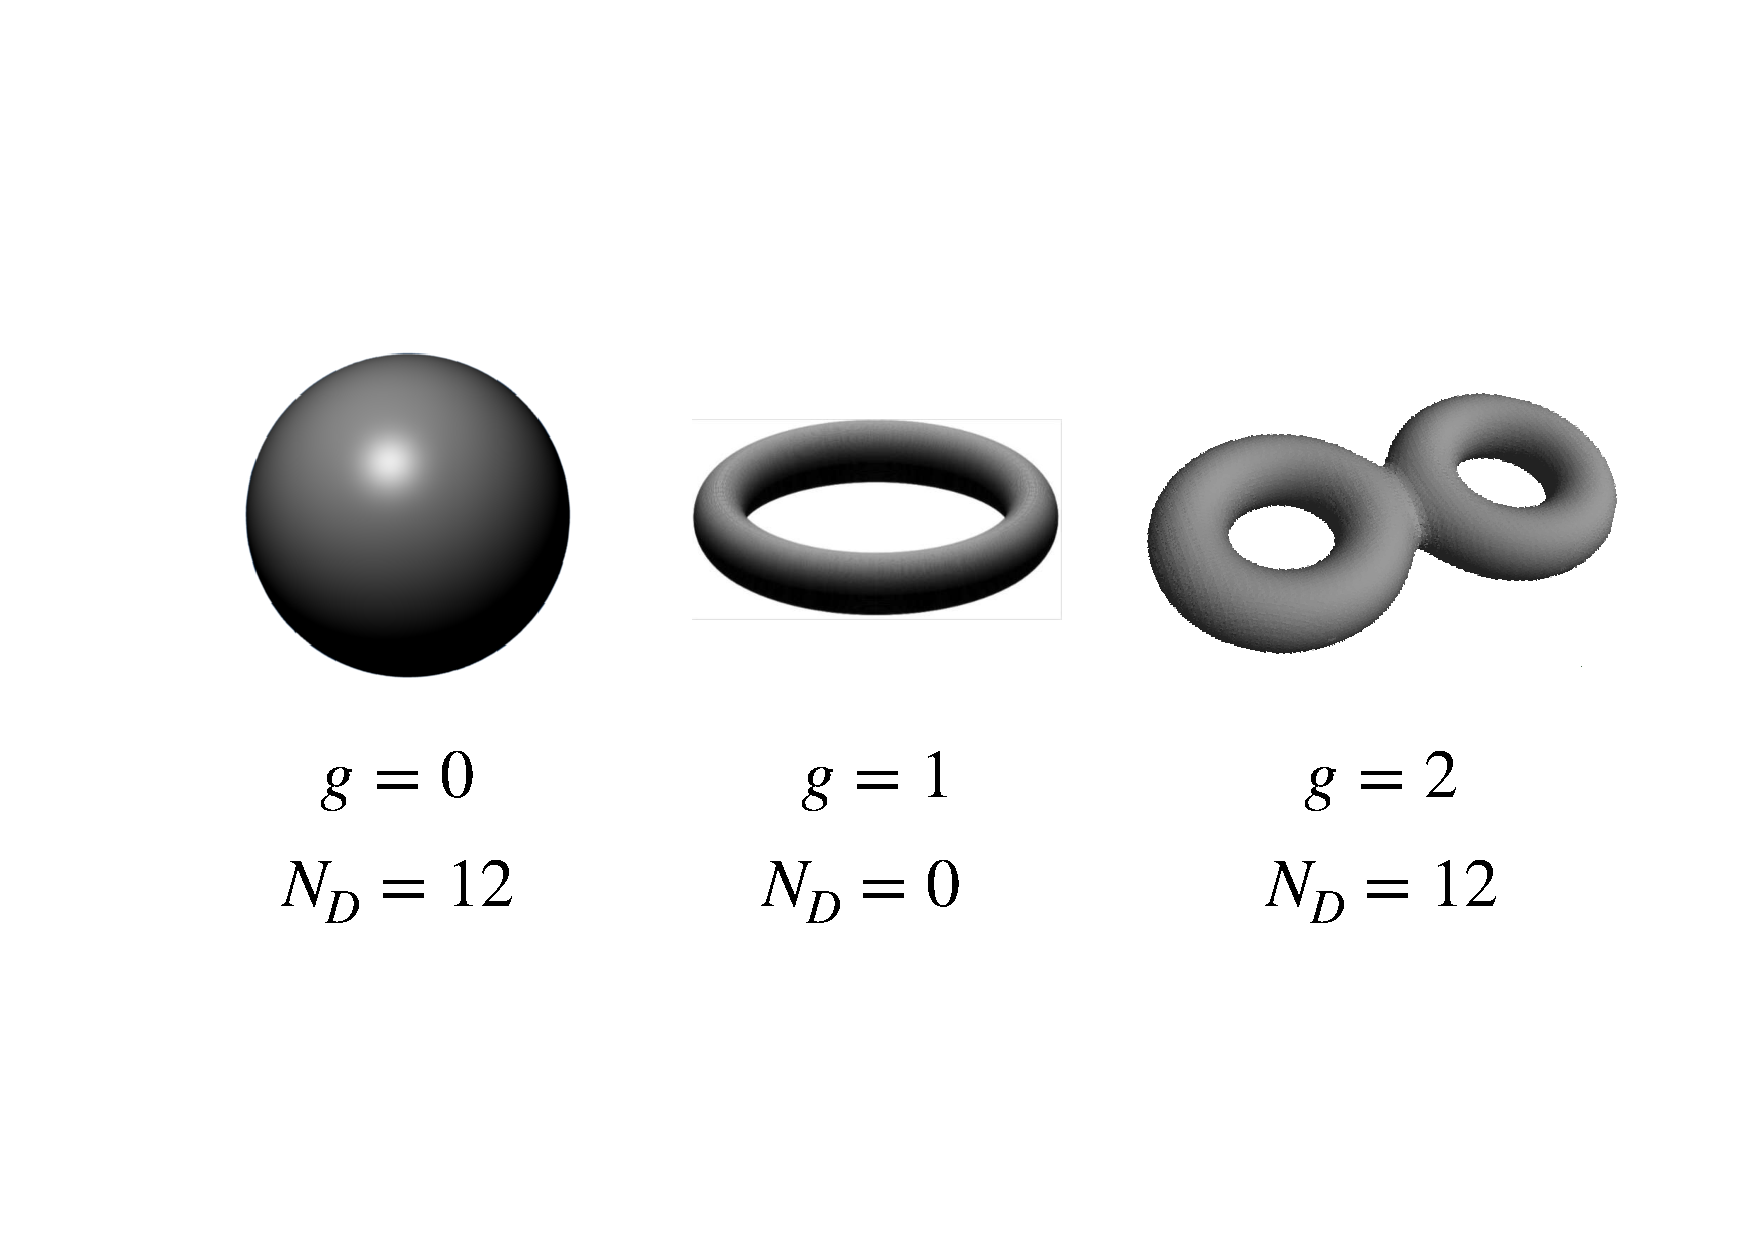
\includegraphics[width=6in]{\MemDiscr/Pics/genus.pages.pdf}
\caption{
۳ مثال از سطوح بسته به همراه جینوس و کمترین تعداد نقاط نقص لازم  برای ساخت آن با مش مثلثی.
}
\label{fig:genus}
\end{center}
\end{figure}


معادلات
\ref{eq:stretchdiscenergy}
و
\ref{eq:bendingdiscenergy}
تغییر انرژی کششی و خمشی یک مش منظم پس از اضافه شدن نقص به مرکز شبکه را توصیف می‌کنند. رقابت میان این دو جمله تعیین می‌کند که یک مش مثلثی کروی به لحاظ انرژی چه شکلی را به خود می‌گیرد. با مقایسه‌ی این دو جمله می‌توان عدد بی بعد  فاپل فون کارمان
\LTRfootnote{Foppl–von Kármán number}
را ساخت
\cite{nelsonPRE2003}
:
\begin{equation}
\gamma = \frac{Y_{2D}R^2}{\kappa}
\label{eq:gamma}
\end{equation}
اگر تمام اضلاع یک مش مثلثی کروی از یک جنس باشند (مدول یانگ و طول اولیه یکسان) در این صورت، عدد فاپل فون کارمان شکل نهایی مش را تایین می‌کند. برای مقادیر زیاد، هزینه‌ی کشش فنر‌ها نسبت به خم شدن بیشتر است و حالت کمینه‌ی انرژی آزاد مجموعه زمانی‌ است که طول تمام اضلاع به طول اولیه‌ خود (انرژی کششی کم) بسیار نزدیک است. از آنجایی که سطح دو بعدی است و قید بسته بودن دارد، به ناچار خمش در محل‌های مشخصی ایجاد می‌شود. از آنجایی که تعداد همسایه‌های مثلث‌های نقاط نقص (۵) کمتر از همسایه‌های مثلث‌های جاهای دیگر (۶) است، هزینه‌ی خم شدن در این نقاط کمتر از جاهای دیگر است و کره شکل بیست‌وجهی
\LTRfootnote{icosehedron}
به خود می‌گیرد.
به همین ترتیب در حد اعداد فاپل فون کارمان کوچک هزینه‌ی کشش در سیستم کم است و سیستم شکل کروی (کمترین خمش) به خود می‌گیرد. در شکل
\ref{fig:gamma}
هندسه‌ی مش مثلثی بسته با ۱۲ نقطه‌ی نقص با گاماهای مختلف نشان داده شده است. در گاماها‌ی کوچک (۴۵) هندسه کروی‌است. این هندسه تا مقدار ۱۵۴ (که مقدار حدی تغییر شکل مش است
\cite{nelsonPRE2003}
) حفظ می‌شود. برای مقادیر گامای بیشتر از ۱۵۴ شکل کره دیگر شکل کمینه‌ی سیستم نخواهد بود و هندسه به طور پیوسته با افزایش گاما به شکل ۲۰ وجهی تغییر می‌کند.
\begin{figure}[h]
\begin{center}
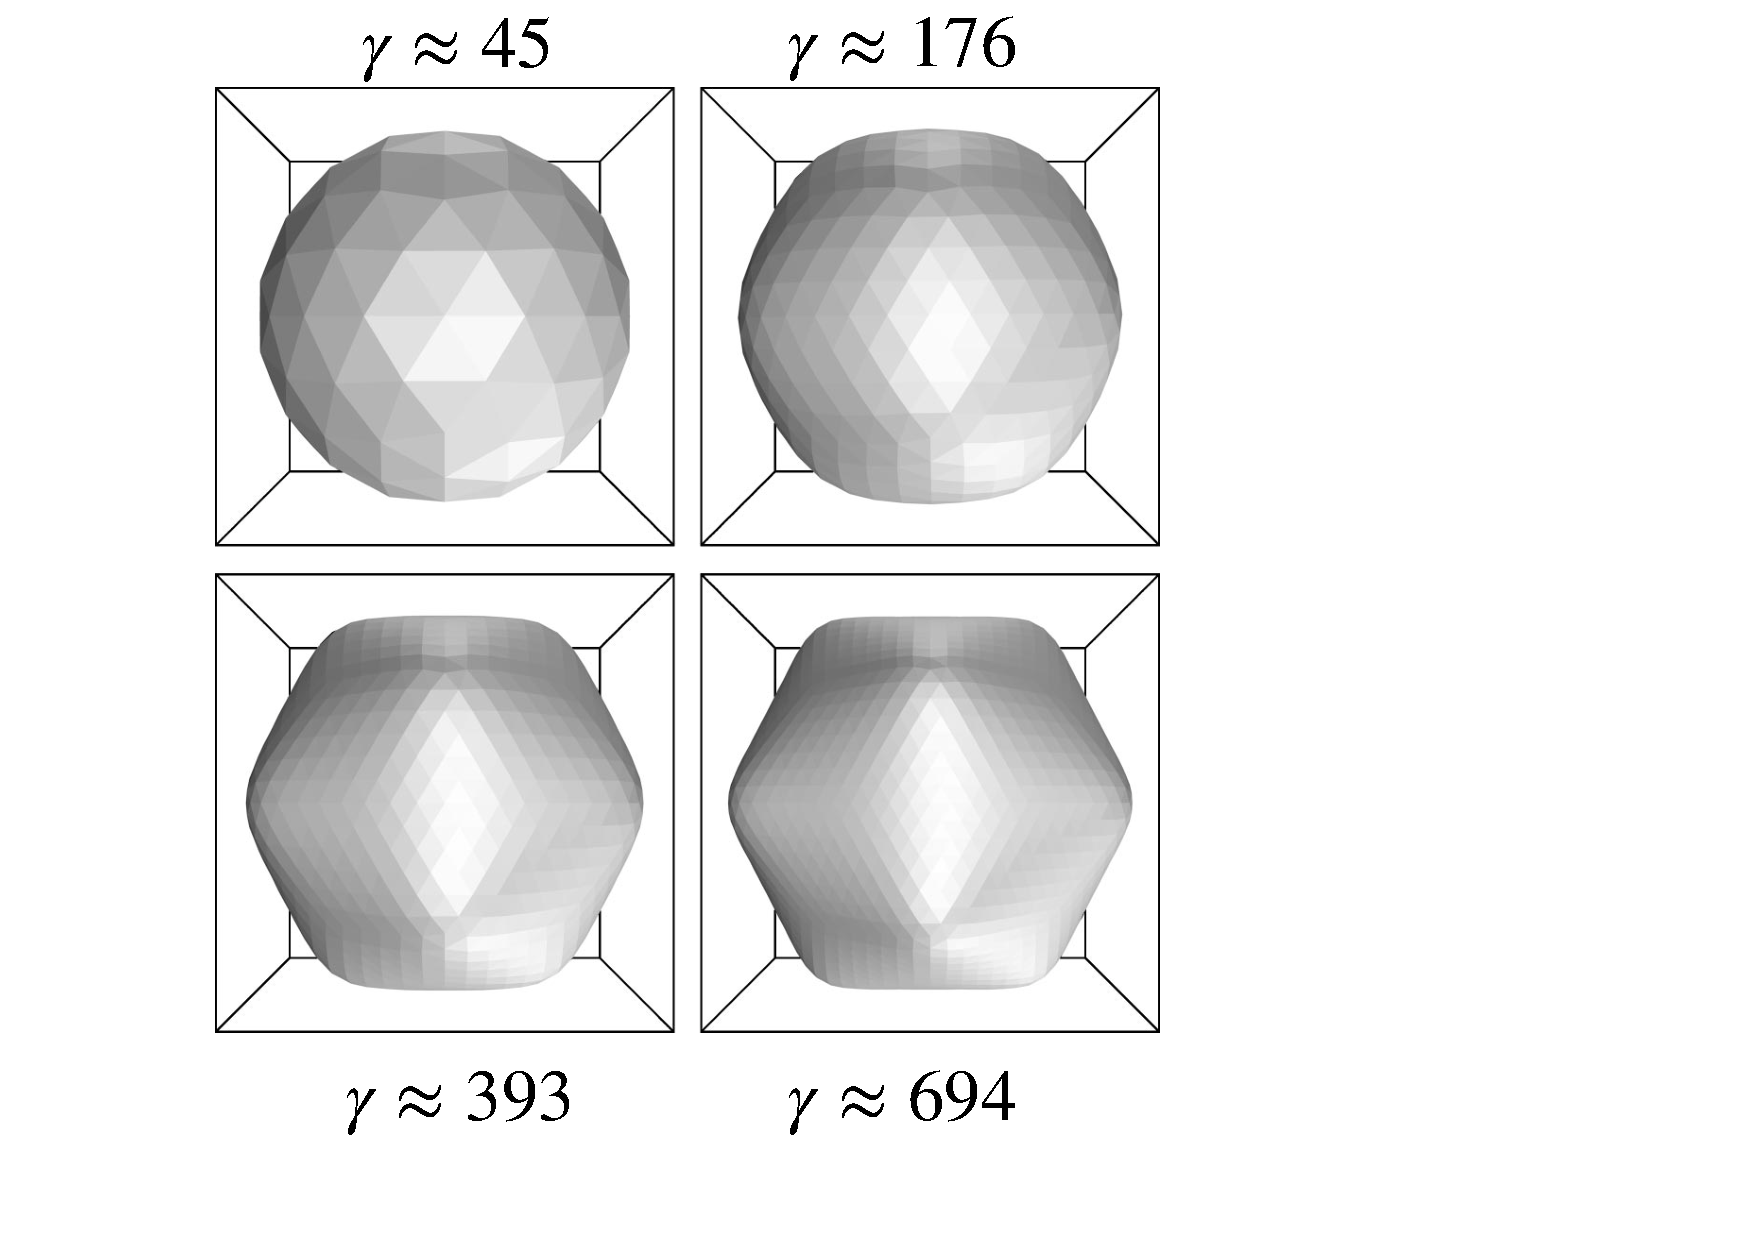
\includegraphics[width=4in]{\MemDiscr/Pics/gamma.pages.pdf}
\caption{
مثال‌هایی از شکل کمینه انرژی مش مثلثی کروی درجه‌ی ۶ با ۱۲ نقطه‌ی نقص. گاما عدد فاپل فون کارمان است. برای مقادیر کم گاما شکل بهینه، کره است و برای مقادیر بالاتر مقدار حدی ۱۵۴، شکل بهینه بیست وجهی است.
}
\label{fig:gamma}
\end{center}
\end{figure}
لازم است تاکید شود که گاما به غیر از مدول‌های الاستیک به اندازه‌ی سطح نیز وا بسته است. در نتیجه در صورتی که مش مثلثی با مدول الاستیک مشخصی ساخته شود، با تنظیم اندازه‌ی مش (یا طول اضلاع) شکل بهینه‌ی سیستم را می‌توان تغییر داد.









%\section{
%الگوریتم مثلث‌بندی دینامیک
%}
%\begin{figure}[h]
\begin{center}
\includegraphics[width=\columnwidth]{\MemMethod/Pics/dynamicTri}
\caption{
تغییر مثلث بندی مِش با تغییر موضعی جفت مثلث‌ها میان چهار نقطه. در حالت اولیه (سمت چپ) دو مثلث با رئوس
$ABC$
و
$DBC$
تعریف شده‌است. با تغییر ضلع مشترک بین دو مثلث از 
$BC$
به
$AD$
مثلث بندی جدید با رئوس
$BAD$
و 
$CAD$
تشکیل خواهد شد (سمت راست).
}
\label{fig:dynamicTri}
\end{center}
\end{figure}



روش  مثلث بندی دینامیک\LTRfootnote{dynamic triangulation}
ابتدا توسط دیوید بول\LTRfootnote{David Boal}
و همکارش 
\cite{Boal1992PRA}
در سال ۱۹۹۲برای مِش‌های مثلثی طراحی شد. هدف اصلی این روش، شبیه‌سازی رفتار سیال گون غشا با استفاده از شبکه‌های مثلثی بود. کمی‌ بعد در همان سال، گامپر و کرول با  شبیه‌سازی موفق غشاهای سیال گون، سبب محبوبیت این روش شدند 
\cite{Gompper1992Science}.
این روش را بسیار محبوب کرد. گامپر و کرول در این مطالعه از روش انحنای دو سطحی برای محاسبه‌ی انرژی انحنا استفاده کردند. همانطور که در بخش
\ref{sec:curvatureDiscDef}
توضیح داده شد، این روش برای محاسبه‌ی انحنای غلط است. در سال ۱۹۹۶ گامپر و کرول روش محاسبه‌ی ایتزیکسون را با روش مثلث بندی دینامیکی ترکیب کردند و با موفقیت رفتار سیال‌گون غشا را شبیه‌سازی کردند
\cite{gompper1996}.

در روش مثلث بندی دینامیک دو مثلث مجاور در نظر گرفته می‌شود. رئوس این دو مثلث مانند شکل 
\ref{fig:dynamicTri}
سمت چپ، چهار وجهی 
$ABCD$
را تشکیل خواهد داد. مثلث بندی در ابتدا دو مثلث 
$ABC$
و
$DBC$
را تعریف می‌کند. با حذف ضلع
$BC$
و ایجاد ضلع
$AD$
مثلث بندی جدید با مثلث‌های
$CAD$
و
$BAD$
تشکیل خواهد شد (شکل
\ref{fig:dynamicTri}
سمت راست). تغییر مثلث بندی، انرژی انحنا و کششی مِش را تغییر خواهد داد. همانطور که در شکل با رنگ‌های قرمز و سبز نمایش داده شده، همسایه‌های مثلث‌های آبی در این فرآیند تغییر خواهد کرد. در نتیجه علاوه بر تغییر زاویه‌ی میان مثلث‌های آبی در دو مثلث بندی، زاویه میان همسایه‌ها نیز تغییر خواهد کرد. به لحاظ انرژی کششی، در صورتی که طول ضلع 
$BC$
و
$AD$
متفاوت باشد، انرژی کششی نیز تغییر خواهد کرد. انتخاب مثلث بندی با یک وزن متروپلیس\LTRfootnote{Metropolis}
 انجام می‌شود. در این روش، ابتدا انرژی مثلث بندی در حالت اولیه محاسبه می‌شود
($E_i$),
سپس مثلث بندی تغییر داده می‌شود و انرژی مش در چیدمان جدید محاسبه ‌می‌شود
($E_f$).
 در صورتی که انرژی با مثلث بندی جدید کاهش پیدا کند مثلث بندی جدید حتما پذیرفته می‌شود. در صورتی که انرژی مثلث بندی جدید بیشتر باشد این چیدمان با یک وزن بولتزمن\LTRfootnote{Boltzman}
انتخاب یا رَد خواهد شد. 

به علت ماهیت این الگوریتم بهترین روش برای شبیه‌سازی آن استفاده از روش مانتی کارلو\LTRfootnote{Monte Carlo}
است. گامپر و کرول هنگام ترکیب الگوریتم مثلث بندی دینامیک با روش اندازه‌گیری انحنای ایتزیکسون، محدودیت‌های زیادی در انتخاب طول اضلاع قرار داد. نتیجه‌ی این محدودیت‌ها ایجاد توزیع یکنواخت نقاط بر سطح شبکه‌ی مثلثی و کنترل شکل و اندازه مثلث‌ها در جهت پایدار کردن روش ایتزیکسون بود.

\begin{figure}[h]
\begin{center}
\includegraphics[width=13cm]{\MemMethod/Pics/DT.pdf}
\caption{
نمایش یک مربع (a)، یک مستطیل (b)، و دو شکل غیر مرتبط (c) که همگلی از ۳۴۰ مثلث متساوی الاضلاع تشکیل شده‌اند.
}  
\label{fig:meshDT}
\end{center}
\end{figure} 


همچنین با استفاده از الگوریتم مثلث‌بندی دینامیک 
\cite{Boal1992PRA, Gompper1992Science},
می‌توان اتصالات مختلف
 $\cal G$
را نمونه‌گیری کرد. این الگوریتم مهم‌ترین و پر کاربرد‌ترین روش برای بازسازی مش است که برای شبیه‌سازی اشکال غشا‌ها استفاده می‌شود. با تعمیم این روش
\cite{Kohyama2003PRE},
می‌توان رفتارهای پیچیده‌ی سطوح مایع‌گون (شکل 
\ref{fig:meshDT}c)
 را نیز شبیه‌سازی کرد. با وجود آزادی زیادی که این روش برای مدل سازی غشا‌ها در اختیار ما قرار می‌دهد، این روش محدودیت‌هایی نیز دارد. قدرت اصلی این الگوریتم در تغییر اتصالات مش‌های سخت است. یعنی برای یک تغییر شکل ساده مربعی به مستطیلی (شکل 
\ref{fig:meshDT})
 باید چیدمان نقاط (و اتصالات میانشان) را با دینامیک موضعیِ پخشی تغییر داد. این کار بسیار زمانبر است.


















